\chapter{Setup and Methods}\label{ch:hardware}

\section{Hardware}

For the vision part a Logitech c920 HD Pro model camera has been used, as seen in Figure \ref{fig:cam}. The camera has Full HD which permits 1080p recordings. Moreover, its five-element glass lens with autofocus gives consistent high definition.

In the case of the robot, an Adept Cobra model has been used, as shown in Figure \ref{fig:cobra}. This robot has 4-axis with 3 rotational joints and one translational (z-axis) joint which operates fast and precisely, at the expense of workspace area. 

\begin{figure}[H]
	\hfill
	\subfigure[Logitech c920 Camera]{
		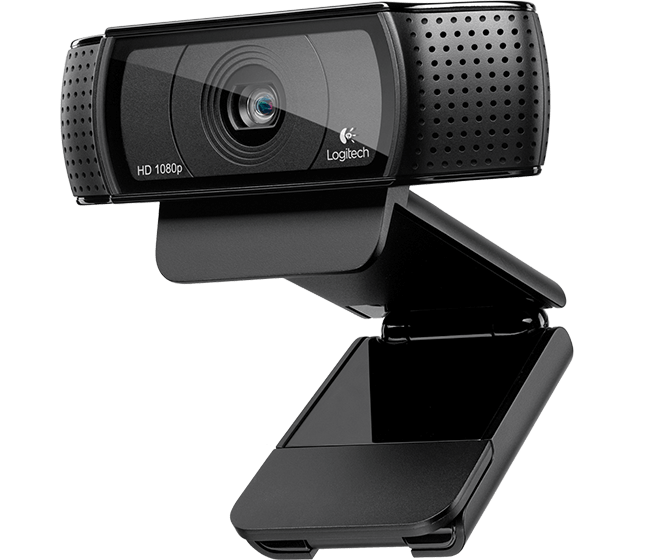
\includegraphics[scale=0.25]{figures/c920.png}
		\label{fig:cam}}
	\hfill
	\subfigure[Adept Cobra Robot]{
		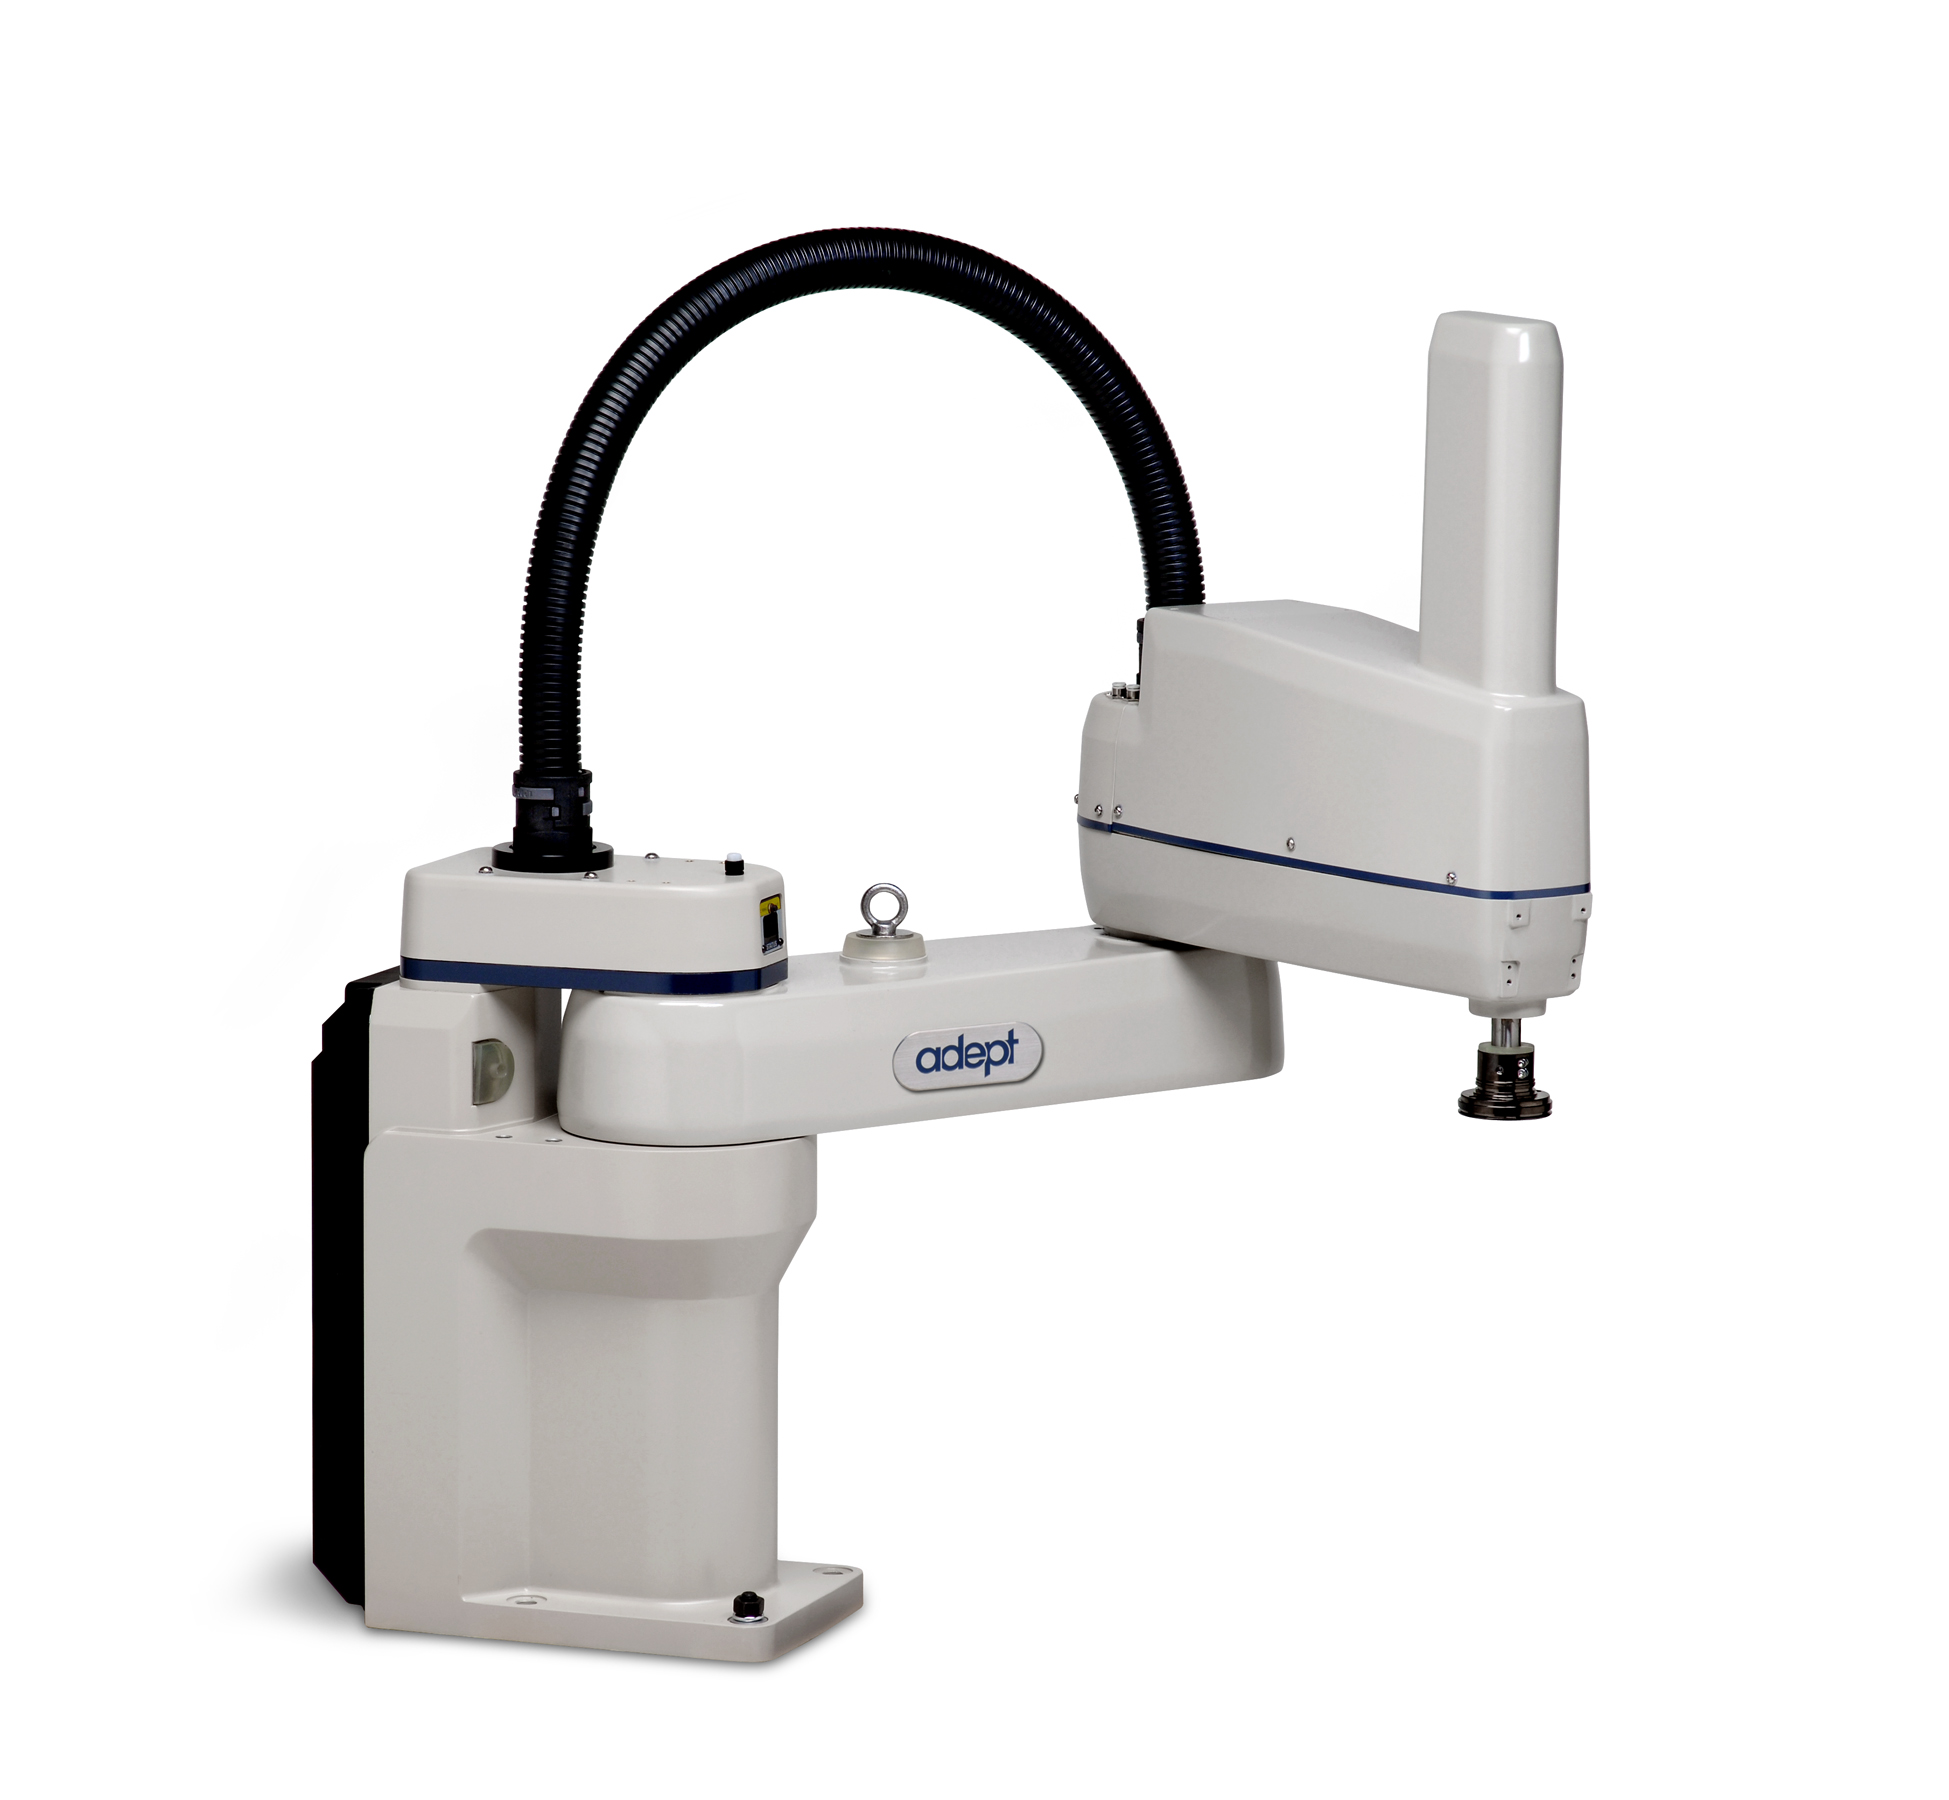
\includegraphics[scale=0.4]{figures/cobra.jpg}
		\label{fig:cobra}}
	\caption{Hardware components}
\end{figure}

A personal computer has been used to connect with the camera and the robot. The camera was placed inside the robot cell, above the blocks, such that the images were taken from the top. This zenithal point of view allows to efficiently determine the positions and orientations of the blocks. 

The physical connections to the computer were made through: 
\begin{itemize}
	\item Ethernet to the robot  
	\item USB to the camera 
\end{itemize}

\begin{figure}[H]
	\centering
	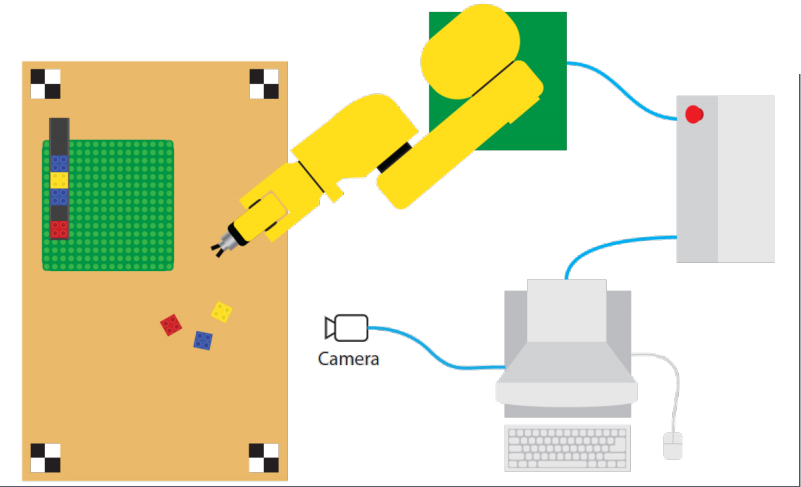
\includegraphics[scale=0.4]{figures/robotCellDesign.png}
	\caption{An illustration of the hardware setup}
\end{figure}

In order to connect between the different components described above, a local network was set up in which both the computer and the Adept Cobra controller were given a static IP. This computer runs the Adept Desktop program that was used to send the instructions to the robot. This configuration allowed us to communicate with the robot and send MATLAB commands to it. MATLAB also includes a camera toolbox to work with it. 

\section{Working principle}\label{sec:workiing_principle}

A thorough explanation of the system's working principle is presented in the following steps:   
\begin{enumerate}
	\item Loading intrinsic and extrinsic parameters.
	\item Create projective matrix by using the previous parameters.
	\item Taking picture of the current workspace.
	\item Crop workspace image. 
	\item Substract background.
	\item Threshold (segmentation) and filter image.
	\item Calculate edges and choose the "biggest" block.
	\item Calculate the centroid and the angle, based on the slope of the block's side.
	\item Translate the image coordinates of the chosen block to the world and robot coordinates.
	\item Move the robot to the calculated position with its respective angle and pick the block.
	\item Move the robot to the building board and drop the block.
	\item Repeat steps 3-11 until the selected figure is finished. Note that the height of the position in the building board will be different depending on how many iterations have been carried out before.
\end{enumerate}